% !Mode:: "Tex:UTF-8"
\chapter{分布式计算理论基础}
    本章主要介绍有关分布式计算模型的一些基础理论知识。我们将首先介绍消息传递系统形式模型,包括异步和同步两种消息传递系统,之后我们会讨论在系统可容错情况下的故障模型。

    \section{消息传递系统}
    在消息传递系统中,处理器之间的通信通过在通信信道上发送消息实现。每个信道在两个特定的处理器之间建立一条双向连接。通信信道的连接情况描述了系统的拓扑结构。系统拓扑由一个无向图表示,其中每个节点代表一个处理器,当且仅当两个节点所对应的处理器之间存在信道时,这两个节点之间的边才存在。我们目前只考虑系统拓扑为连通图的情况。通常,我们将信道的集合称为网络。具有特定拓扑的消息传递系统中,一个算法由系统中的每个处理器的本地程序组成。一个处理器的本地程序使得处理器能够执行本地计算,向给定拓扑中的邻居发送消息,以及接收来自邻居的消息。
    \begin{figure}[ht]
        \centering
        % Requires \usepackage{graphicx}
        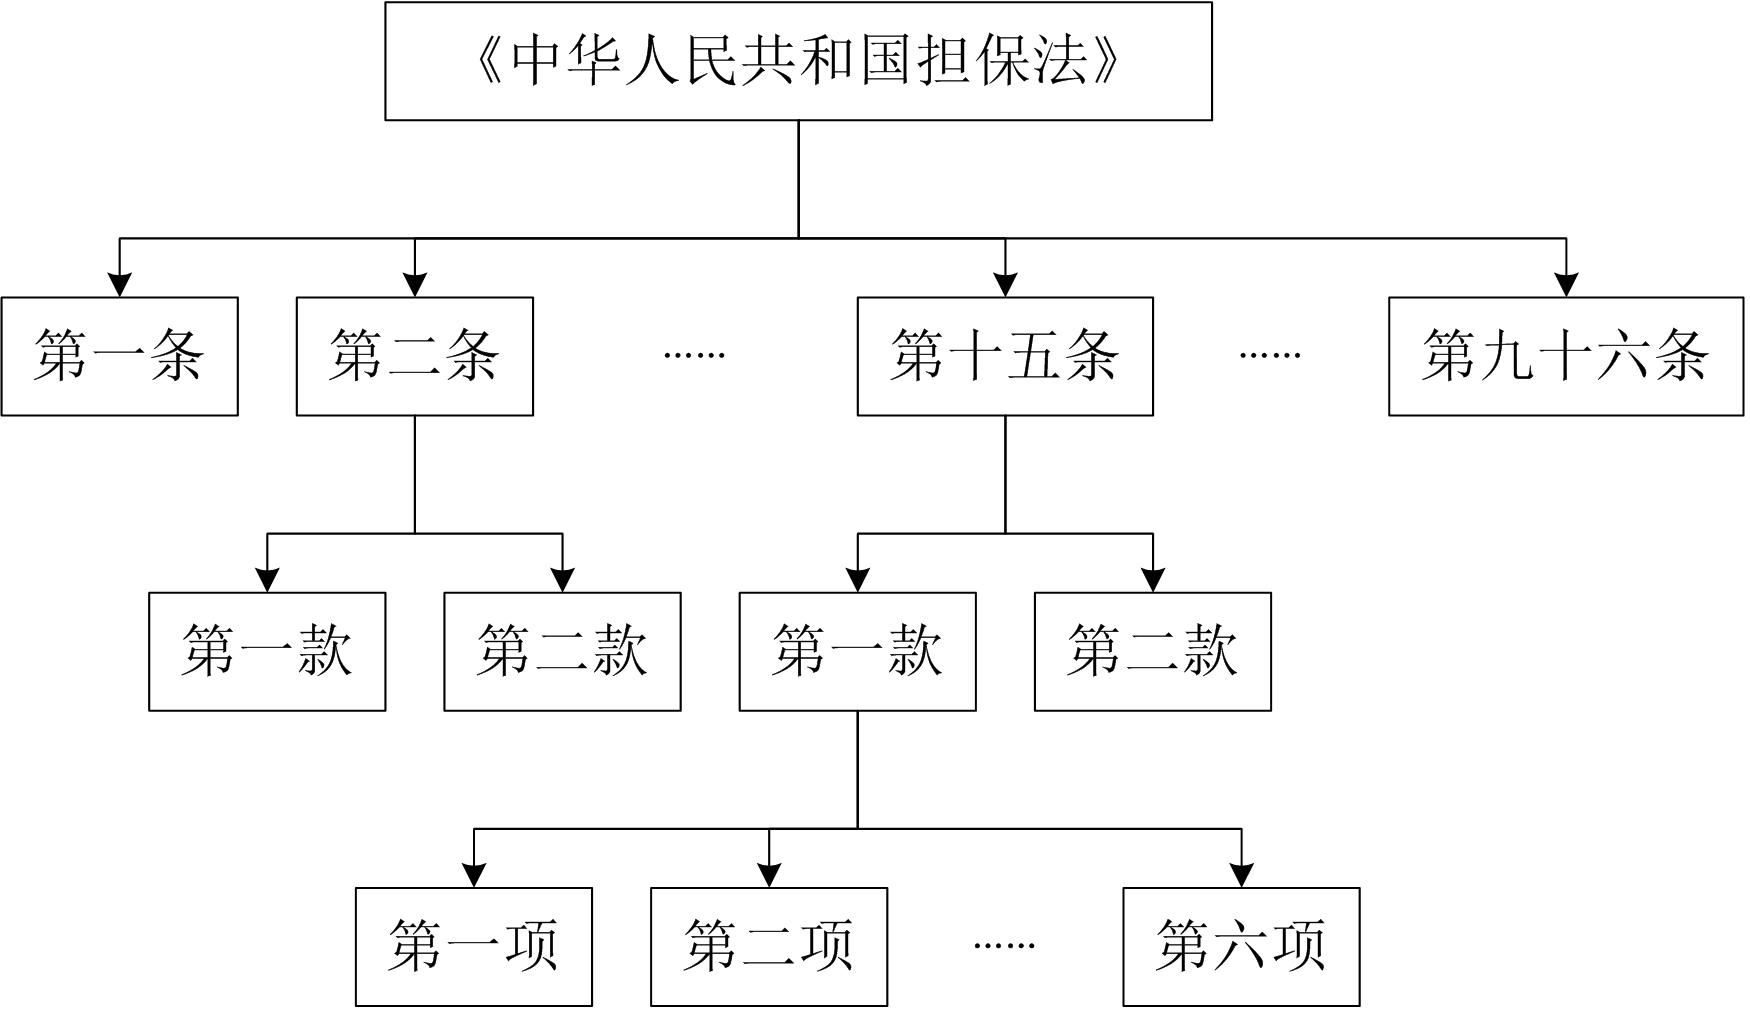
\includegraphics[width=10cm]{Figure1}\\
        \caption{一个简单的拓扑图}\label{Figure1}
    \end{figure}

    更正式地讲,一个系统或者算法由$n$ 个处理器$p_0,...,p_{n-1}$ 组成,其中$i$ 是处理器 $p_i$ 的索引。每个处理器$p_i$ 被建模为一个(可能是无限的)状态机,其状态集合为$Q_i$\cite{lynch1981describing}。一个处理器在拓扑图中被标识为一个特定的节点。拓扑图中与处理器$p_i$ 邻接的边被随机标注为整数$1$ 到$r$,其中$r$ 是$p_i$ 的度(见图\ref{Figure1})。处理器$p_i$ 的每个状态包含$2r$ 个特殊组件,$outbuf_i[l]$ 和$inbuf_i[l]$,其中每个$l$ 均满足$1 \leq l \leq r$。 这些特殊的组件是消息的集合:$outbuf_i[l]$ 保存了$p_i$ 通过第$l$ 条邻接信道发送给邻居但是尚未被交付的消息,$inbuf_i[l]$ 保存了通过第$l$ 条邻接信道交付给$p_i$ 但是$p_i$ 尚未通过内部计算步骤进行处理的消息。状态集合$Q_i$ 含有一个特殊的子集$\pozhehao$初始状态。在初始状态中,每个$inbuf_i[l]$ 必须为空,而$outbuf_i[l]$ 组件并不需要。

    处理器的状态,除去$outbuf_i[l]$ 组件,组成了$p_i$ 的可容许状态(admissible state)。当向$p_i$ 的可容许状态输入一个值时,处理器$p_i$ 的转换函数开始执行。执行的结果是为$p_i$ 的可容许状态输出一个值,该状态中每个$inbuf_i[l]$ 为空。执行的结果也可能是为每一个$1$ 到$r$ 之间的$l$ 输出最多一条消息:这就是将要发送给在$p_i$ 的第$l$ 条邻接信道另一端的邻居的消息。因此,$p_i$ 之前发送并等待交付的消息不会影响$p_i$ 当前的步骤;每个步骤处理所有等待交付给$p_i$ 的消息并且引发状态的改变,同时会向每个邻居最多发送一条消息。

    一个配置(configuration)是一个矢量$C=(q_0,...,q_{n-1})$ ,其中$q_i$ 是$p_i$ 的一个状态。一个配置中$outbuf$ 的状态表示了通信信道上正在传送的消息。一个初始配置是一个矢量($q_0,...q_{n-1}$),其中每个$q_i$ 是$p_i$ 的一个初始状态,也就是说,每个处理器都处在初始状态。

    系统中能够发生的动作被建模为事件。对于消息传递系统,我们考虑两种事件。一种是计算事件,表示为$comp(i)$, 代表处理器$p_i$ 的一次计算步骤,该步骤中$p_i$ 的转换函数会应用到它当前的可容许状态。另一种是交付事件,表示为$del(i,j,m)$,代表消息$m$ 从处理器$p_i$ 发送到$p_j$。

    系统随时间的行为被建模为执行(execution),即为一个配置和事件相交替的序列\cite{owicki1976axiomatic}。这个序列要满足各种各样的条件,这些条件由被建模系统的特定类型决定。我们将这些条件分为安全性和活跃性条件两类。安全性条件要求序列的每个有限前缀都要满足;比如,“处理器$p_i$ 的每一个步骤之后都跟随着处理器$p_0$ 的一个步骤。”非正式地讲,安全性条件声明了系统中还没有坏事发生;比如刚刚给的例子可以重新描述为要求$p_1$ 的一个步骤之后绝不会跟随着除了$p_0$ 之外的其他处理器的一个步骤。活跃性条件是必须保持一个特定次数,可能是无限次的条件。例如,条件“$p_1$ 进行无限次步骤”需要条件“$p_1$ 刚刚进行一次步骤”必须重复发生无限次。非正式地讲,活跃性条件表示最终有些好事发生。满足一个特定系统类型要求的所有安全性条件的任意序列可以称为执行。如果一个执行也满足所有要求的活跃性条件,那么它是可容许的\cite{fischer1985impossibility}。

    下面我们来定义同步和异步这两种消息传递系统中的执行和可容许执行需要满足的条件。

    \subsection{异步消息传递系统}
    对于一个系统,如果消息传递花费的时间以及处理器的连续步骤间的时间间隔没有固定的上限,那么这个系统就称为是异步的。异步系统的一个例子就是因特网,消息(比如E-mail)可能会过几天才能到达,尽管这经常只需要数秒。通常消息延迟和处理器步骤时间间隔会有上限,但是有时候这些上限会很大,只会在极少的情况下达到,而且会随着时间变化。我们通常需要设计独立于任何时间参数而不是依赖于这些限制的算法,也就是异步算法。

    异步消息传递系统中的一个执行片段$\alpha$ 是一个如下形式的(有穷或者无穷的)序列:
    \begin{center}
    $C_0,\phi_1,C_1,\phi_2,C_2,\phi_3,...$
    \end{center}

    其中每个$C_k$ 是一个配置,每个$\phi_k$ 是一个事件。如果$\alpha$ 是有限的,那么它必须以一个配置结束。进一步地,以下条件必须满足:
    \begin{itemize}
      \item 如果$\phi_k=del(i,j,m)$,那么$m$ 必须是$C_{k-1}$ 中$outbuf_i[l]$ 的一个元素,其中$l$ 是$p_i$ 赋予信道$\{p_i,p_j\}$ 的标签。从配置$C_{k-1}$ 到$C_k$ 的唯一变化是$m$ 从$C_{k-1}$ 中的$outbuf_i[l]$ 中移除,同时$m$ 被加入到$C_k$ 中的$inbuf_j[h]$,其中$h$ 是$p_j$赋予信道$\{p_i,p_j\}$ 的标签。总之,一条消息被交付当且仅当它处于发送状态,并且发生的唯一变化是把消息从发送方的输出缓冲移动到接收方的输入缓冲。
      \item 如果$\phi_k=comp(i)$,那么从$C_{k-1}$ 到$C_k$ 的唯一变化是$p_i$ 根据其作用于$C_{k-1}$ 中$p_i$ 的可容许状态上的转换函数改变状态,同时由$p_i$的转换函数确定的消息集合会被加入到$C_k$ 中的$outbuf_i$ 参数中。这些消息被称作在这个事件中被发送。总之,$p_i$ 基于其当前状态由转换函数(本地程序)改变状态并发送消息,当前状态包含了待交付的消息(但不包括待发送消息)。处理器的转换函数会保证$inbuf$ 变量会被清空。
    \end{itemize}

    一个执行(execution)是一个执行片段$C_0,\phi_1,C_1,\phi_2,C_2,\phi_3,...$,其中$C_0$ 是初始配置。

    对于每个执行(或者执行片段)我们关联一个计划(或者计划片段),所谓计划(schedule)即为执行中事件的序列,$\phi_1,\phi_2,\phi_3,...$。不是每个事件序列都能与每个初始配置相匹配:比如,$del(1,2,m)$ 不是$outbufs$ 为空的初始配置的一个计划,因为没有$p_1$ 的之前的步骤能导致$m$ 被发送。注意如果本地程序是确定性的,那么执行(或者执行片段)就只由初始(或开始)配置$C_0$ 和计划(或者计划片段)$\sigma$ 决定,表示为$exec(C_0,\sigma)$。

    在异步模型中,一个执行是可容许的当且仅当每个处理器都执行无穷次计算事件并且发送的每条消息都最终被交付。要求无穷次计算事件模拟了处理器不会发生故障的事实。它不代表处理器的本地程序必须包含一个无限循环;一个算法结束的非正式概念可以调整为一旦处理器完成了它的任务,使其转换函数在一个特定的点之后不再改变处理器的状态。换句话说,处理器在那个时间点之后执行“假步骤”。如果一个计划是一个可容许执行的计划,那么它是可容许的。

    \subsection{同步消息传递系统}
    在同步系统中,处理器按照锁步(lockstep)执行:一个执行被分割成若干时间片,在每个时间片,每个处理器可以向每个邻居发送一条消息,所有消息将被交付,之后每个处理器会根据刚刚收到的消息进行计算。这种模型,在实际的分布式系统中尽管通常无法达到,但是对于算法设计非常方便,因为算法不需要考虑很多不确定性。当一个算法针对这一理想的时间模型设计之后,可以自动模拟到其他更为现实的时间模型中工作,正如我们接下来将要看到的一样。

    正式地讲,同步情况下执行的定义比起异步情况下的定义有了进一步的限制,其定义如下。间隔的配置和事件可以被分割成不相交的周期(round)。 一个周期包含了$outbuf$ 变量中所有消息的一次交付事件,直到所有的$outbuf$ 变量为空,紧接着所有处理器进行一次计算。因此,一个周期包含了如下过程:首先交付所有待发送的消息,然后让所有的处理器进行一次内部计算步骤来处理所有交付了的消息。

    同步模型中,如果一个执行是无限的,那么它是可容许的。由于周期的结构,这意味着每个处理器进行无限次计算步骤,并且每条发送的消息最终都会被交付。在异步的情形下,假定可容许执行是无限的是为了追求技术上的便利;同步情形下算法的终止可以像异步情形中一样处理。

    注意在没有故障的同步系统中,一旦算法确定,执行能够不同的唯一影响因素是初始配置。在异步系统中,同一算法会有很多不同的执行,即便是初始配置相同且没有故障,这是因为处理器步骤之间可以交叉并且消息延迟是不确定的。

    \section{故障模型}
    当分布式系统不可靠时,会产生很多新的问题。对于同步消息传递系统中的良性故障,一个错误的处理器会崩溃,也就是停止运行,但是不会执行错误的操作(例如交付尚未被发送的消息)。我们研究一个基本的协同问题$\pozhehao$协商问题,它需要所有的处理器根据它们的(可能冲突的)输入达成一个共同的输出。还是在同步消息传递系统中,错误的处理器可能产生有更为严重的错误行为。我们假定故障是拜占庭的(Byzantine),也就是一个发生故障的处理器的行为是任意的。在这种情况下如果要解决协商问题,错误的处理器数量不能多于总数的三分之一。而在异步系统中,一个确定性算法无法解决协商问题,即便只有一个处理器以简单崩溃的形式发生故障。不管通信是以消息传递还是共享读写变量实现,这一结论都成立。

    我们要讨论的是容错分布式计算中的一个简单例子:一个同步系统,其中处理器会以简单地停止运行方式发生故障。我们假定对于我们讨论的所有消息传递系统,其通信拓扑图是完全的,即处理器都处于一个环的节点上。更进一步地,我们假定通信信道完全可依赖,所有发送的消息都将被交付。

    为了应对处理器崩溃的情况,我们需要修改同步消息传递系统中一些形式定义。在定义中一个至关重要的参数是$f$,也即能够失效的处理器的最大数量。我们称这样的系统是$f-resilient$ 的。

    在系统可靠的情况下,同步系统的一个执行由一系列的周期组成。在每一周期,$outbuf$ 变量中的所有消息都会被交付,然后所有处理器都将进行一次运算。而对于一个$f-resilient$ 系统,一个执行的定义修改如下。存在一个包含$f$ 个处理器的子集$F$,即错误处理器集合。错误处理器集合在不同执行中可能不同,因此我们无法提前知道哪个处理器是错误的。在每个周期中,每个不在$F$ 中的处理器都正好有一次计算事件,而在$F$ 中的处理器最多有一次计算事件。更进一步地,如果$F$ 中的某个处理器在某个周期没有计算事件,那么在任何后继周期中也不会有计算事件。最后,在一个错误处理器执行计算事件的最后一个周期,其输出消息集合中的一个随机子集会被发送\cite{attiya2004distributed}。
